\begin{spacing}{1.5}
\phantom
\phantom
\phantom
\phantom
\section{Results}
\phantom
\phantom
\noindent From the method outlined in \emph{Chapter 4}, the following statistics were derived for the study area (i.e., fires in ecoregions 3E, 3W and 3S, over the period 1989--2004).

\subsection{Total Number of Forest Fires}

The number of new forest fires--per year ($N_{\mathrm{t}}$), \emph{Table~\ref{tab3}}, was calculated by aggregating the total number of data points (in this case, the final size of each fire), in each year (see \emph{Appendix B: 1.4} for calculations); \\





% latex table generated in R 2.15.0 by xtable 1.7-0 package
% Sun Aug 26 10:10:13 2012
\begin{table}[ht]
\begin{center}
\begin{tabular}{|r|r|}
  \hline
Year & Fires \\ 
  \hline
1989 & 478 \\ 
  1990 & 323 \\ 
  1991 & 736 \\ 
  1992 & 219 \\ 
  1993 & 113 \\ 
  1994 & 303 \\ 
  1995 & 771 \\ 
  1996 & 508 \\ 
  1997 & 506 \\ 
  1998 & 755 \\ 
  1999 & 293 \\ 
  2000 & 194 \\ 
  2001 & 430 \\ 
  2002 & 361 \\ 
  2003 & 395 \\ 
  2004 & 144 \\ 
   \hline
\end{tabular}
\caption[The number of forest fires--per year (Nt)]{\emph{The number of forest fires--per year (Nt)}}
\label{tab3}
\end{center}
\end{table}

\noindent The total number of forest fires ($N$) was then calculated by aggregating ($N_{\mathrm{t}}$); \\

\noindent $N$ = 6525 fires.

\clearpage

\noindent Therefore, we can say that in the study area there were a total of 6,529 fires, over the period 1989--2004. Of those fires, the vast majority, 5607 (86\%), were suppressed (via Initial Attack) before becoming >3 ha in size. 744 (11\%) fires were put out by continued suppression (i.e., fires >3ha but <200 ha), and only 178 (3\%) escaped continued suppression, (i.e., burning >200 ha of forest).

\subsection{Area Burned by Forest Fires}

The area burned by forest fires, per year ($A_{\mathrm{t}}$), \emph{Table~\ref{tab4}}, was calculated by aggregating the final size of every fire, per year (see \emph{Appendix B: 1.4} for calculations): \\


% latex table generated in R 2.15.0 by xtable 1.7-0 package
% Sun Aug 26 10:10:13 2012
\begin{table}[ht]
\begin{center}
\begin{tabular}{|r|r|}
  \hline
Year & Area (ha) \\ 
  \hline
1989 & 17615 \\ 
  1990 & 3584 \\ 
  1991 & 19876 \\ 
  1992 & 10244 \\ 
  1993 & 18483 \\ 
  1994 & 2336 \\ 
  1995 & 158269 \\ 
  1996 & 236434 \\ 
  1997 & 22459 \\ 
  1998 & 45144 \\ 
  1999 & 138822 \\ 
  2000 & 632 \\ 
  2001 & 1268 \\ 
  2002 & 14759 \\ 
  2003 & 103703 \\ 
  2004 & 172 \\ 
   \hline
\end{tabular}
\caption[The area burned by forest fires, per year (At)]{\emph{The area burned by forest fires, per year (At)}}
\label{tab4}
\end{center}
\end{table}
\noindent The total area burned by forest fires ($A$) over the study period is therefore, the summation of ($A_{\mathrm{t}}$): \\


\noindent A = 793797 ha \\

\clearpage

\noindent These result can also be interpreted graphically by taking the mean area burned per year, as shown in \emph{Figure~\ref{fig9}}, (see \emph{Appendix B: 1.5} for calculations). \\

\begin{figure}[h!]
  \centering
    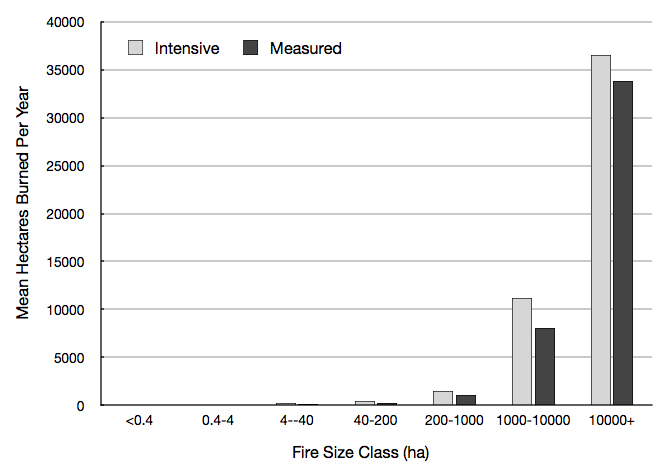
\includegraphics[width=1\textwidth]{media/fig9}
      \caption[Mean hectares burned by size class]{\emph{Mean hectares burned by size class (1989--2004) in the Intensive and Measured fire management zones.}}
        \label{fig9}
\end{figure}

\noindent These results are consistent with Cumming's (2005:2) observation (see \emph{Chapter 3.1}) that fires greater that 200 ha, account for the vast majority  of the area burned by forest fires every year (98\% in this case). Hence, why preventing fires from becoming this large is a primary concern for fire managers in Ontario.

\subsection{Fire Size Distributions}

In Ward and Tithecott's (1993) original analysis (see \emph{Chapter 2.1}), the authors used the relative fire size distributions in different fire management zones as an indicator of the impact of fire suppression in Ontario. They predicted that an area with aggressive fire suppression would have fewer large fires, than an area without. \\

\noindent To see how this prediction has fared over the period 1989--2004, the fire size distributions (measured as a percentage of fires in that zone) were calculated (see \emph{Appendix B 1.1-1.3} for calculations). The results of those calculations are shown in \emph{Figure~\ref{fig10}}, on page~\pageref{fig10}.

\clearpage

\begin{figure}[h!]
  \centering
    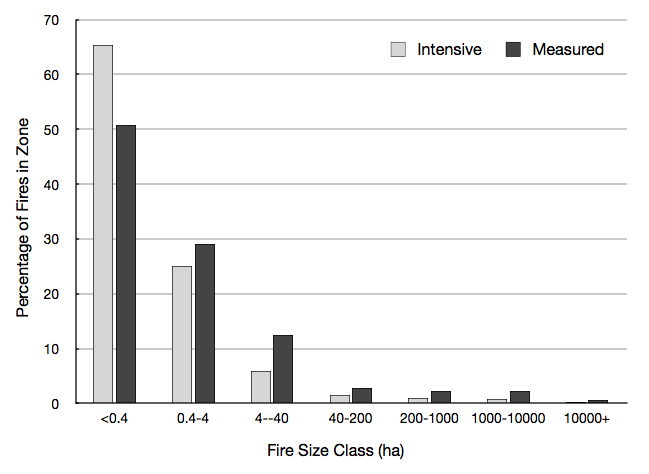
\includegraphics[width=.8\textwidth]{media/fig10}
      \caption[Percentage of fires by size class]{\emph{Percentage of fires by size class (1989--2004) in the Intensive and Measured fire management zones.}}
        \label{fig10}
\end{figure}

\noindent While it is not readily apparent, there is indeed a significant difference in the fire size distributions between the Intensive and Measured fire management zones. If we focus in on fires at the large end of the size class spectrum (see \emph{Figure~\ref{fig11}}), it can clearly be shown that there is approximately twice the number of moderate-- and large--sized fires (i.e., fires >40 ha) in the Measured zone compared to the Intensive zone. \\

\begin{figure}[h!]
  \centering
    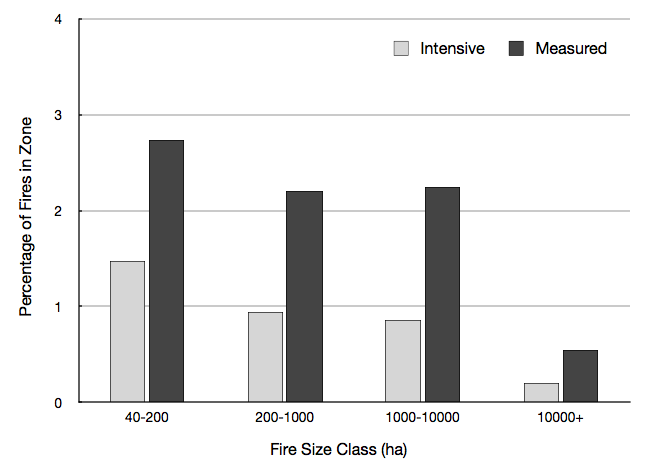
\includegraphics[width=.8\textwidth]{media/fig11}
      \caption[Percentage of fires for size classes 40 ha to 10000+ ha]{\emph{Percentage of fires for size classes 40 ha to 10000+ ha (1989--2004) in the Intensive and Measured fire management zones.}}
        \label{fig11}
\end{figure}

\noindent From the analysis presented above, one might be tempted to draw the same conclusion as Ward and Tithecott (1993), that aggressive fire suppression in the Intensive zone has lead to far fewer moderate-- and large--sized fires. However, this would be based on the counter factual-- that without fire suppression the fire size distribution in the Intensive zone would have been the same as that of the Measured zone. Therefore, while these results are certainly indicative of the impact fire suppression has had, it can not alone, prove the effectiveness of fire suppression in Ontario.

\subsection{The Generalised Liner Model}

To measure the effectiveness of fire suppression in a more scientifically robust manner, a generalised liner model (GLM) was developed (see \emph{Chapter 4.3}), that would not only estimate the suppression probabilities between the fire management zone, but also control for other environmental factors that may be influencing the distribution of forest fires in Ontario. \\

\noindent The suppression probability ($p$) in both the Intensive and Measured zones were estimated using the generalised liner model (GLM) as follows: \\

\texttt{glm.eq =} ''\texttt{cbind(suppressed, unsuppressed)} $~$ \texttt{zone + ecoregion}'' \\

\texttt{glm(glm.eq, family=binomial(logit), data=omnr.glm) }\\

\noindent The results of which, can then be displayed using the \texttt{summary()} function: \\

\noindent \texttt{summary(glm.out)} \\

\noindent The results of which are detailed in \emph{Table~\ref{tab5}}. \\


% latex table generated in R 2.15.0 by xtable 1.7-0 package
% Sun Aug 26 10:10:13 2012
\begin{table}[ht]
\begin{center}
\begin{tabular}{r|rrrr}
  \hline
 & Estimate & Std. Error & z value & Pr($>$$|$z$|$) \\ 
  \hline
(Intercept) & 1.6691 & 0.1819 & 9.18 & 0.0000 \\ 
  zonemea & -0.0043 & 0.1822 & -0.02 & 0.9813 \\ 
  ecoregionS3 & 0.0101 & 0.2751 & 0.04 & 0.9708 \\ 
  ecoregionW3 & -0.7142 & 0.2150 & -3.32 & 0.0009 \\ 
   \hline
\end{tabular}
\caption[Coefficients for the GLM (zone + ecoregion)]{\emph{Coefficients for the Generalised Liner Model (zone + ecoregion)}}
\label{tab5}
\end{center}
\end{table}

\subsection{Interpreting the GLM}

The way in which the \texttt{glm()} command works is to estimate the suppression probability ($p$) in the (\texttt{intensive zone / ecoregion 3E}) as default and then add the other interaction terms sequentially-- as follows; (\texttt{measured zone / ecoregion 3E}), (\texttt{intensive zone / ecoregion 3S}), (\texttt{measured zone / ecoregion 3S}), (\texttt{intensive zone / ecoregion 3W}), (\texttt{measured zone / ecoregion 3W}). \\

\noindent The last coefficient (\texttt{ecoregion 3W}) in the summary, therefore shows the estimate, standard error and significance value for the complete model. \\

\noindent The estimate is reported as -0.7142, however this is a log of odds. Therefore, to find the suppression probability ($p$) (as an odds ratio), it must first be interpreted as the antilog of the model estimate: \\

\noindent \texttt{exp}(-0.7142) $=$ $p$\\

\noindent $p$ $=$ 0.4896 \\
                
\noindent Therefore; \\
 
\noindent \textbf{All else being equal (i.e., when interaction with the ecoregion variable is controlled), the odds of a fire being suppressed in the Measured zone is less than half (0.5) that of the Intensive zone, giving the Intensive zone a significant advantage in terms of fire suppression effectiveness.}

\subsection{Measuring the Performance of the Model}
The performance of the model can be evaluated in two distinct ways, via ANOVA and AIC.

\subsubsection{ANOVA}
ANOVA (analysis of variance) is often used to analyse the results of experiments by testing for statistical significance. The results outlined above, may be called statistically significant if they are unlikely to have occurred by chance alone. A calculated probability is used to determine if this is true. If the probability is less than a pre--determined threshold, called a significance level (usually 0.05, i.e., 5\% chance), we can safely reject the null hypothesis. By testing hypotheses in this way, we can significantly limit Type \texttt{I} errors (i.e., false positives). \\

\noindent In this case, the null hypothesis $H_{\mathrm{0}}$, is that there is no difference between the fire suppression probabilities of the Intensive and Measured fire management zones (in statistics this usually means that all the results are samples of the same population). This implies that the different fire management strategies have no discernible effect on the resulting fire suppression probabilities. Ergo, rejecting the null hypothesis would imply that the different fire management strategies \emph{have} in fact altered fire suppression probabilities. \\

\noindent Testing the results will be operationalised as a chi square test, which will show how well the interaction terms (zone and ecoregion) explain the deviation between the model and the data. \\

\noindent The advantage of statistical programming is that the output of the generalised liner models is saved as a single vector (glm.out), which can then easily be used in further analysis. Therefore, while a chi square test can often be complicated to implement, it can be programmed in R simply using the following command: \\

\noindent \texttt{anova(glm.out, test="Chisq")} \\

\noindent The results of which are detailed in \emph{Table~\ref{tab6}}. \\

% latex table generated in R 2.15.0 by xtable 1.7-0 package
% Sun Aug 26 10:10:14 2012
\begin{table}[ht]
\begin{center}
\begin{tabular}{r|rrrrr}
  \hline
 & Df & Deviance & Resid. Df & Resid. Dev & Pr($>$Chi) \\ 
  \hline
NULL &  &  & 5 & 26.92 &  \\ 
  zone & 1 & 0.60 & 4 & 26.32 & 0.4381 \\ 
  ecoregion & 2 & 17.19 & 2 & 9.12 & 0.0002 \\ 
   \hline
\end{tabular}
\caption[Analysis of variance for the GLM (zone + ecoregion)]{\emph{Analysis of variance for the Generalised Liner Model (zone + ecoregion)}}
\label{tab6}
\end{center}
\end{table}
\noindent The results of the chi square test show the null deviance to be 26.92 points on 5 degree of freedom. This number represents how well the response variable (number of fires suppressed) is predicted by the model with only the intercept. Adding in the interaction terms (\texttt{zone} and \texttt{ecoregion}) decreased this deviance by 17.2 points on 2 degree of freedom. When interpreted as a chi square value (0.00018), it indicates a highly significant decrease in deviance (where <0.05 is considered to be statistically significant). This gives us a >99\% confidence interval in that these results are not due to random chance alone. While these values are computed automatically in R, it is still possible to use F tables in the Engineering Statistics Handbook (Croarkin and Tobias 2003) and look up these values by hand. \\

\noindent One should note however, that this test rests upon one key assumption about the data. That is in the independence of each observation (Snedecor and Cochran 1967:321). In this case, independence means that each forest fire needs to be an independent event. However, fire ecologists may point out that forest fires (and the suppression of those fires) may change the distribution of subsequent fires (i.e., that suppressing a fire today, simply adds more fuel for fires to burn in the future). While this is undoubtably the case, modelling this behaviour is far beyond the scope of this project and, therefore, for the sake of simplicity, independence was assumed. \\

\noindent From the generalised liner model we have found the suppression probabilities ($p$) in the Intensive and Measured zones to be different by a ratio of 2 to 1. By analysing of variance of this model, we now know that this deviation can be explained by the different suppression strategies employed in each fire management zone. Therefore, the null hypothesis $H_{\mathrm{0}}$ was rejected.

\subsubsection{AIC}

The Akaike Information Criterion (AIC) was developed by Hirotsugu Akaike (1974), and is used to test a goodness of fit of a statistical model. The AIC also takes into account the tradeoff between the accuracy and complexity of the model. This is done by penalising a model for increasing the number of interaction terms, thereby, discouraging over--fitting (i.e., adding spurious covariates simply to increase the goodness of fit). However, the AIC value only provides a relative measure of fit, and can therefore, only be used as a method for choosing between competing models (rather than hypothesis testing). \\

\noindent The AIC value is derived from the following equation; \\

\noindent \texttt{AIC} = 2$k$ -- 2\texttt{ln}($L$) \\

\noindent Where; \\

\begin{tabular}{ll}
$k$ is the number of interaction terms used \\
$L$ is the maximum value of the likelihood of the model \\
\end{tabular}\\ \\

\noindent Therefore, given several different models that may explain the data, the model with the lowest AIC value is preferred. In \emph{Chapter 4.4}, the different models used were outlined as model $S$ (strategy) and model $SE$ (strategy + ecoregion), (*Note model $0$ (null) has already been rejected). \\

\noindent The AIC values for these models are as follows; \\

\begin{tabular}{ll}
model $S$   = 59.14 \\
model $SE$ = 45.95 \\
\end{tabular}\\

\noindent As such, model $SE$ (i.e., the full model used in the ANOVA test above) best fits the data.

\subsection{The Temporal Model}
To test the effect temporal variation has on the dataset, a further generalised liner model was developed, that estimates the suppression probability ($p$) in both the Intensive and Measured zones, on an annual basis. The GLM was coded as follows: \\

\texttt{glm.eq =} ''\texttt{cbind(suppressed, unsuppressed)} $~$ \texttt{zone + load}'' \\

\texttt{glm(glm.eq, family=binomial(logit), data=omnr.glm) }\\ \\

\noindent The results of which are detailed in \emph{Table~\ref{tab7}}, on page~\pageref{tab7}. \\

\clearpage


% latex table generated in R 2.15.0 by xtable 1.7-0 package
% Sun Aug 26 10:10:14 2012
\begin{table}[ht]
\begin{center}
\begin{tabular}{r|rrrr}
  \hline
 & Estimate & Std. Error & z value & Pr($>$$|$z$|$) \\ 
  \hline
(Intercept) & 1.9210 & 0.1895 & 10.14 & 0.0000 \\ 
  zonemea & -0.9464 & 0.1377 & -6.87 & 0.0000 \\ 
  load & 0.0001 & 0.0001 & 1.00 & 0.3192 \\ 
   \hline
\end{tabular}
\caption[Coefficients for the GLM (zone + load)]{\emph{Coefficients for the Generalised Liner Model (zone + load)}}
\label{tab7}
\end{center}
\end{table}
\noindent A chi square test was aslo performed to see if the load interaction term explained the deviation (\emph{Table~\ref{tab8}}). \\

% latex table generated in R 2.15.0 by xtable 1.7-0 package
% Sun Aug 26 10:10:14 2012
\begin{table}[ht]
\begin{center}
\begin{tabular}{r|rrrrr}
  \hline
 & Df & Deviance & Resid. Df & Resid. Dev & Pr($>$Chi) \\ 
  \hline
NULL &  &  & 31 & 238.46 &  \\ 
  zone & 1 & 44.03 & 30 & 194.43 & 0.0000 \\ 
  load & 1 & 0.99 & 29 & 193.44 & 0.3188 \\ 
   \hline
\end{tabular}
\caption[Analysis of variance for the GLM (zone + load)]{\emph{Analysis of variance for the Generalised Liner Model (zone + load)}}
\label{tab8}
\end{center}
\end{table}
\noindent The results of the chi square test show the null deviance to be 238 points on 31 degree of freedom. This is a very large deviance. Adding in the interaction term (\texttt{zone}) decreased this deviance by 44 points on 30 degree of freedom. Further more, adding the interaction term (\texttt{load}), only reduced this deviance by 1 point on 29 degree of freedom. When interpreted as a chi square value (0.32), it indicates a very low decrease in deviance (where <0.05 is considered to be statistically significant). This gives us no confidence in the results of this model. In addition, the AIC value of model $SL$ = 295.8, which is very high, suggesting that the model is not a good fit. \\

\noindent This analysis suggest that fire suppression is not confounded, to any significant degree, by the annual number of fires in each zone. Therefore, the only parsimonious conclusion from the evidence presented here, is that the difference in fire management strategies between the intensive and measured zone has been primarily responsible for the observed differences in fire distributions over the period 1989--2004 and, as such, the aggressive fire suppression strategy employed by the OMNR can be considered effective at reducing the number of large forest fires in Ontario.

\end{spacing}
\clearpage
